\documentclass[supercite]{Experimental_Report}

\title{~~~~~~数据结构实验~~~~~~}
\author{刘欣逸}
\school{计算机科学与技术学院}
\classnum{CS2210}
\stunum{U202115473}
\instructor{郑渤龙}
\date{2023年5月29日}


\usepackage{ctex}
\usepackage{listings}
\usepackage{placeins}
\usepackage{algorithm, multirow}
\usepackage{algpseudocode}
\usepackage{amsmath}
\usepackage{amsthm}
\usepackage{framed}
\usepackage{mathtools}
\usepackage{subcaption}
\usepackage{xltxtra} %提供了针对XeTeX的改进并且加入了XeTeX的LOGO, 自动调用xunicode宏包(提供Unicode字符宏)
\usepackage{bm}
\usepackage{tikz}
\usepackage{tikzscale}
\usepackage{pgfplots}
\usepackage{enumitem}

\usepackage{xcolor}
\definecolor{commentColor}{RGB}{53,129,34}
\definecolor{keywordColor}{RGB}{172, 62, 158}
\definecolor{stringColor}{RGB}{194, 62, 42}
\definecolor{preprocessorColor}{RGB}{114, 75, 48}
\definecolor{characterColor}{RGB}{31, 53, 207}
\definecolor{numberColor}{RGB}{166, 166, 166}
\definecolor{oglobalColor}{RGB}{97, 64, 154}
\definecolor{globalColor}{RGB}{89, 127, 134}
\definecolor{functionColor}{RGB}{56,36,124}

\usepackage{fontspec}
\newfontfamily\sfr{SFMono-Regular}
\newfontfamily\sfb{SFMono-Bold}

\usepackage{listings}
\lstset{
	language=C++,
	basicstyle=\sffamily\sfr,
	keywordstyle=\color{keywordColor}\sffamily\sfr,
	commentstyle=\color{commentColor}\sffamily\sfr,
	stringstyle=\color{stringColor}\sffamily\sfr,
	showstringspaces=false,
	columns=fullflexible,keepspaces,
	numbers=left,
	numberstyle=\color{numberColor}\footnotesize\sfr,
	escapechar=\$,
	morecomment=*[s][\color{stringColor}\sffamily\sfr]{<}{>},
	morecomment=[s][\color{characterColor}\sffamily\sfr]{'}{'},
	keywords=[2]{std, cout, cin},
	keywordstyle = [2]{\color{oglobalColor}\sffamily\sfr},
	keywords=[3]{endl, printf, scanf, setw, setfill, setbase, setprecision, time, ctime, rand},
	keywordstyle = [3]{\color{functionColor}\sffamily\sfr},
	keywords=[4]{\#include},
	keywordstyle =[4]{\color{preprocessorColor}\ssfamily\sfr},
	literate={
		{<<}{{{\color{black}<<}}}1
		{>>}{{{\color{black}>>}}}1
		{*}{{{*}}}1
		{0}{{{\color{characterColor}0}}}1
		{1}{{{\color{characterColor}1}}}1
		{2}{{{\color{characterColor}2}}}1
		{3}{{{\color{characterColor}3}}}1
		{4}{{{\color{characterColor}4}}}1
		{5}{{{\color{characterColor}5}}}1
		{6}{{{\color{characterColor}6}}}1
		{7}{{{\color{characterColor}7}}}1
		{8}{{{\color{characterColor}8}}}1
		{9}{{{\color{characterColor}9}}}1
		},
	tabsize=4,
	frame=single,
	frameround=tttt
}


\pgfplotsset{compat=1.16}

\newcommand{\cfig}[3]{
  \begin{figure}[htb]
    \centering
    \includegraphics[width=#2\textwidth]{images/#1.tikz}
    \caption{#3}
    \label{fig:#1}
  \end{figure}
}

\newcommand{\sfig}[3]{
  \begin{subfigure}[b]{#2\textwidth}
    \includegraphics[width=\textwidth]{images/#1.tikz}
    \caption{#3}
    \label{fig:#1}
  \end{subfigure}
}

\newcommand{\xfig}[3]{
  \begin{figure}[htb]
    \centering
    #3
    \caption{#2}
    \label{fig:#1}
  \end{figure}
}

\newcommand{\rfig}[1]{\autoref{fig:#1}}
\newcommand{\ralg}[1]{\autoref{alg:#1}}
\newcommand{\rthm}[1]{\autoref{thm:#1}}
\newcommand{\rlem}[1]{\autoref{lem:#1}}
\newcommand{\reqn}[1]{\autoref{eqn:#1}}
\newcommand{\rtbl}[1]{\autoref{tbl:#1}}

\algnewcommand\Null{\textsc{null }}
\algnewcommand\algorithmicinput{\textbf{Input:}}
\algnewcommand\Input{\item[\algorithmicinput]}
\algnewcommand\algorithmicoutput{\textbf{Output:}}
\algnewcommand\Output{\item[\algorithmicoutput]}
\algnewcommand\algorithmicbreak{\textbf{break}}
\algnewcommand\Break{\algorithmicbreak}
\algnewcommand\algorithmiccontinue{\textbf{continue}}
\algnewcommand\Continue{\algorithmiccontinue}
\algnewcommand{\LeftCom}[1]{\State $\triangleright$ #1}

\newtheorem{thm}{定理}[section]
\newtheorem{lem}{引理}[section]

\colorlet{shadecolor}{black!15}

\theoremstyle{definition}
\newtheorem{alg}{算法}[section]

\def\thmautorefname~#1\null{定理~#1~\null}
\def\lemautorefname~#1\null{引理~#1~\null}
\def\algautorefname~#1\null{算法~#1~\null}

\begin{document}

\maketitle

\clearpage

\pagenumbering{Roman}

\tableofcontents[level=2]

\clearpage

\pagenumbering{arabic}

\section{基于顺序存储结构的线性表实现}


\subsection{问题描述}


要求构造一个具有菜单的功能演示系统。该演示系统实现多个线性表管理。其中,在主函数中准备函数调用所需实参值、显示函数执行结果,并给出适当的操作提示。

实现依据最小完备性和常用性相结合的原则确定的初始化表、销毁表、清空表、判定空表、求表长和获得元素等12种基本运算,具体运算功能定义如下。
\begin{enumerate}


	\item 初始化表:函数名称是\verb|InitaList(L)|;初始条件是线性表\verb|L|不存在已存在;操作结果是构造一个空的线性表。


	\item 销毁表:函数名称是\verb|DestroyList(L)|;初始条件是线性表\verb|L|已存在;操作结果是销毁线性表\verb|L|。


	\item 清空表:函数名称是\verb|ClearList(L)|;初始条件是线性表\verb|L|已存在;操作结果是将\verb|L|重置为空表。


	\item 判定空表:函数名称是\verb|ListEmpty(L)|;初始条件是线性表\verb|L|已存在;操作结果是若\verb|L|为空表则返回\verb|TRUE|,否则返回\verb|FALSE|。


	\item 求表长:函数名称是\verb|ListLength(L)|;初始条件是线性表\verb|L|已存在;操作结果是返回\verb|L|中数据元素的个数。


	\item 获得元素:函数名称是\verb|GetElem(L,i,e)|;初始条件是线性表\verb|L|已存在, \\ \verb|1<=i<=ListLength(L)|;操作结果是用\verb|e|返回\verb|L|中第\verb|i|个数据元素的值。


	\item 查找元素:函数名称是\verb|LocateElem(L,e,compare())|;初始条件是线性表\verb|L|已存在;操作结果是返回\verb|L|中第一个与\verb|e|满足关系\verb|compare()|关系的数据元素的位序,若这样的数据元素不存在,则返回值为\verb|0|。


	\item 获得前驱:函数名称是\verb|PriorElem(L,cur_e,pre_e)|;初始条件是线性表\verb|L|已存在;操作结果是若\verb|cur_e|是\verb|L|的数据元素,且不是第一个,则用\verb|pre_e|返回它的前驱,否则操作失败,\verb|pre_e|无定义。


	\item 获得后继:函数名称是\verb|NextElem(L,cur_e,next_e)|;初始条件是线性表\verb|L|已存在;操作结果是若\verb|cur_e|是\verb|L|的数据元素,且不是最后一个,则用\verb|next_e|返回它的后继,否则操作失败,\verb|next_e|无定义。


	\item 插入元素:函数名称是\verb|ListInsert(L,i,e)|;初始条件是线性表\verb|L|已存在,\\ \verb|1<=i<=ListLength(L)+1|;操作结果是在\verb|L|的第\verb|i|个位置之前插入新的数据元素\verb|e|。


	\item 删除元素:函数名称是\verb|ListDelete(L,i,e)|;初始条件是线性表\verb|L|已存在且非空,\verb|1<=i<=ListLength(L)|;操作结果:删除\verb|L|的第\verb|i|个数据元素,用\verb|e|返回其值。


	\item 遍历表:函数名称是\verb|ListTraverse(L,visit())|,初始条件是线性表\verb|L|已存在;操作结果是依次对\verb|L|的每个数据元素调用函数\verb|visit()|。
\end{enumerate}
此外,还在基础功能的基础上实现了附加功能:
\begin{enumerate}

	\item 最大连续子数组和:函数名称是\verb|MaxSubArray(L)|;初始条件是线性表\verb|L|已存在且非空,请找出一个具有最大和的连续子数组(子数组最少包含一个元素),操作结果是其最大和;


	\item 和为\verb|K|的子数组:函数名称是\verb|SubArrayNum(L,k)|; 初始条件是线性表\verb|L|已存在且非空,操作结果是该数组中和为\verb|k|的连续子数组的个数;


	\item 顺序表排序:函数名称是\verb|SortList(L)|;初始条件是线性表\verb|L|已存在;操作结果是将\verb|L|由小到大排序;

	\item 实现线性表的文件形式保存:其中,
	\begin{itemize}
		\item 需要设计文件数据记录格式,以高效保存线性表数据逻辑结构\verb|(D,{R})|的完整信息;
		\item  需要设计线性表文件保存和加载操作合理模式。
	\end{itemize}

	\item 实现多个线性表管理:设计相应的数据结构管理多个线性表的查找、添加、移除等功能。
\end{enumerate}
实验目的:
\begin{enumerate}
	\item 加深对线性表的概念、基本运算的理解;
	\item 熟练掌握线性表的逻辑结构与物理结构的关系;
	\item 物理结构采用顺序表,熟练掌握线性表的基本运算的实现。
\end{enumerate}

\subsection{系统设计}
本系统提供一个采用顺序存储方式的线性表及其操作实现。
系统可供选择的操作有:
\begin{itemize}
	\item 基本操作:初始化线性表、销毁表、清空表、判定空表,求表长、获得元素、查找元素、获得某元素的前驱、获得某元素的后继、插入元素、删除元素、遍历线性表。
	\item 附加功能:最大连续子数组和、和为\verb|K|的子数组、顺序表排序、实现线性表的文件形式保存、实现多个线性表管理。
\end{itemize}

\subsubsection{头文件、宏和类型定义}
\begin{lstlisting}
#include <stdio.h>
#include <stdlib.h>
#include <string.h>
#include <limits.h>

#define TRUE 1
#define FALSE 0
#define OK 1
#define ERROR 0
#define INFEASIBLE -1
#define OVERFLOW -2
#define ISEMPTY -3
#define LIST_INIT_SIZE 1000
#define LISTINCREMENT  10
#define max(i,j) ((i)>(j)?(i):(j))

typedef int status;
typedef int ElemType; //数据元素类型定义
typedef struct{  //顺序表(顺序结构)的定义
    ElemType * elem;
    int length;
    int listsize;
} SqList;

typedef struct THELISTS{  //顺序表的管理表定义
	 struct ALIST{
		 char name[30];
		 SqList L;
	  } elem[50];
	  int length = 0;
	  int listssize = 50;
 } LISTS;
\end{lstlisting}

\subsubsection{函数设计}
\begin{enumerate}
\item 函数名称:\verb|InitaList(L)|;

初始条件:线性表\verb|L|不存在;

操作结果:是构造一个空的线性表;

算法思路:先分配存储空间后,将表长设为\verb|0|,再将线性表容量变量设为预定义的初始存储容量。

\item 函数名称:\verb|DestroyList(L)|;

初始条件:线性表\verb|L|已存在;

操作结果:销毁线性表\verb|L|;

算法思路:释放内存并将其他结构成员设置为初值。

\item 函数名称:\verb|ClearList(L)|;

初始条件:线性表\verb|L|已存在;

操作结果:将\verb|L|重置为空表;

算法思路:将表长设为\verb|0|。

\item 函数名称:\verb|ListEmpty(L)|;

初始条件:线性表\verb|L|已存在;

操作结果:若\verb|L|为空表则返回\verb|TRUE|,否则返回\verb|FALSE|;

算法思路:表长为\verb|0|则为空表,否则不是空。

\item 函数名称:\verb|ListLength(L)|;

初始条件:线性表\verb|L|已存在;

操作结果:返回\verb|L|中数据元素的个数;

算法思路:返回线性表表长的值。

\item 函数名称:\verb|GetElem(L,i,e)|;

初始条件:线性表已存在,\verb|1<=i<=ListLength(L)|;

操作结果:用\verb|e|返回\verb|L|中第\verb|i|个数据元素的值;

算法思路:将线性表中第\verb|i|个数据元素的值赋值给\verb|e|。

\item 函数名称:\verb|LocateElem(L,e,compare())|;

初始条件:线性表已存在;

操作结果:返回线性表中第\verb|1|个与\verb|e|相等的数据元素的位置,若这样的数据元素不存在,则返回值为\verb|0|;

算法思路:从索引低位开始顺序查找,如果找到返回该元素的位序

\item 函数名称:\verb|PriorElem(L,cur_e,pre_e)|;

初始条件:线性表\verb|L|已存在;

操作结果:若\verb|cur_e|是\verb|L|的数据元素并且不是第一个数据元素,用\verb|pre_e|返回它的前驱,否则操作失败。

算法思路:首先判断该元素不是第一个数据元素,再查找该结点,如果查找成功且该结点有前驱元素,则将前驱元素赋值给\verb|pre_e|。若未找到该结点,或者该结点是第一个数据元素,则返回\verb|ERROR|。

\item 函数名称:\verb|NextElem(L,cur_e,next_e)|

初始条件:线性表\verb|L|已存在;

操作结果:若\verb|cur_e|是\verb|L|的数据元素,且不是最后一个,则用\verb|next_e|返回它的后继,否则操作失败,\verb|next_e|无定义。

算法思路:首先判断该元素不是最后一个数据元素,再查找该结点,如果查找成功且该结点有后继元素,则将后继元素赋值给\verb|next_e|。若未找到该结点,或者该结点是最后一个数据元素,则返回\verb|ERROR|。

\item 函数名称:\verb|ListInsert(L,i,e)|

初始条件:线性表\verb|L|已存在且非空,\verb|1<=i<=ListLength(L)+1|;

操作结果:在\verb|L|的第\verb|i|个位置之前插入新的数据元素\verb|e|。

算法思路:先遍历顺序表,若线性表\verb|L|已存在且不为空,输入的\verb|i|值不合法,则返回\verb|ERROR|;若\verb|i|的值合法,则在线性表的第\verb|i|个位置前插入新数据元素\verb|e|,返回\verb|OK|。若线性表\verb|L|不存在,返回\verb|INFEASIBLE|.

\item 函数名称:\verb|ListDelete(L,i,e)|;

初始条件:线性表\verb|L|已存在且非空,\verb|1<=i<=ListLength(L)|;

操作结果:删除\verb|L|的第\verb|i|个数据元素,用\verb|e|返回其值;

设计思想:先遍历顺序表,如果线性表\verb|L|已存在且非空,并且输入的\verb|i|值不合法,则返回\verb|ERROR|。若满足线性表\verb|L|已存在且\verb|L|非空,并且\verb|i|的值合法,则删除线性表的第\verb|i|个位置的数据元素,并用\verb|e|返回其值,返回\verb|OK|。

\item 函数名称:\verb|ListTraverse(L)|;、

初始条件:线性表\verb|L|已存在;

操作结果:依次遍历\verb|L|的每个数据元素;

设计思想:若线性表\verb|L|存在,则依序遍历元素;否则返回\verb|ERROR|。

\item 函数名称:\verb|SaveList(L,filename)|;

初始条件:线性表\verb|L|已存在;

操作结果:将线性表\verb|L|保存到指定文件;

算法思路:用\verb|fprintf|保存为文件。

\item 函数名称:\verb|LoadList(L)|;

初始条件:文件\verb|filename|已存在;

操作结果:从文件中加载数据到\verb|L|;

算法思路:用\verb|fscanf|将文件读取顺序表。

\item 函数名称:\verb|MaxSubArray(L)|;

初始条件:线性表\verb|L|已存在;

操作结果:返回线性表\verb|L|的最大连续子数组和;

算法思路:逐个枚举子数组求出最大连续子数组和。

\item 函数名称:\verb|SubArrayNum(L,k)|;

初始条件:线性表\verb|L|已存在;

操作结果:返回线性表\verb|L|的和为k的连续子数组个数;

算法思路:逐个枚举子数组求出和为k的连续子数组个数。

\item 函数名称:\verb|SortList(L)|

初始条件:线性表\verb|L|已存在;

操作结果:将\verb|L|中的元素按升序排序;

算法思路:用冒泡排序算法将\verb|L|的数据元素按升序排序。

\end{enumerate}

\subsection{系统实现}

见《附录A 基于顺序存储结构线性表实现的源程序》。

\subsection{系统测试}
先用插入操作创建包含元素1、2、3、4、5、6、7的顺序表。再测试判空、查找、删除、遍历、销毁等基础功能。
\begin{enumerate}
\item \verb|InitList()|
	\begin{figure}[!htb]
		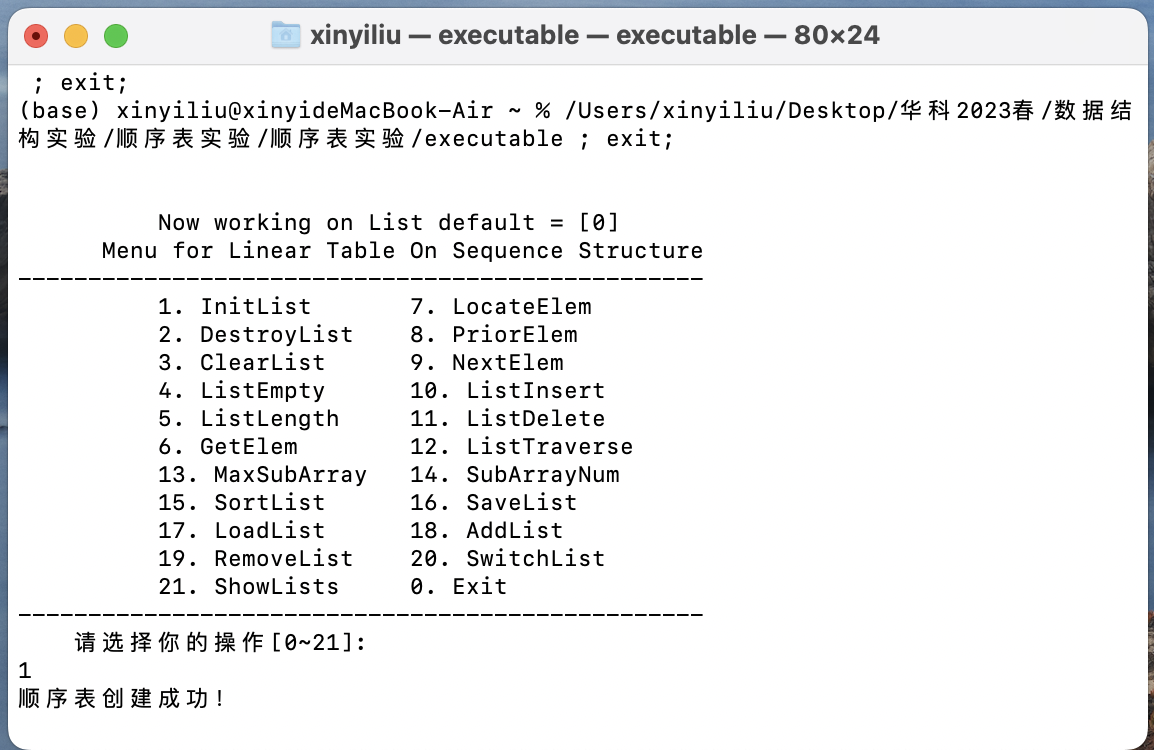
\includegraphics[width=0.8\linewidth]{images/截屏2023-06-01 18.21.29.png}
	\end{figure}
\FloatBarrier

\item \verb|ListInsert()|
	依次插入了元素1、2、3、4、5、6、7。
	\begin{figure}[!htb]
		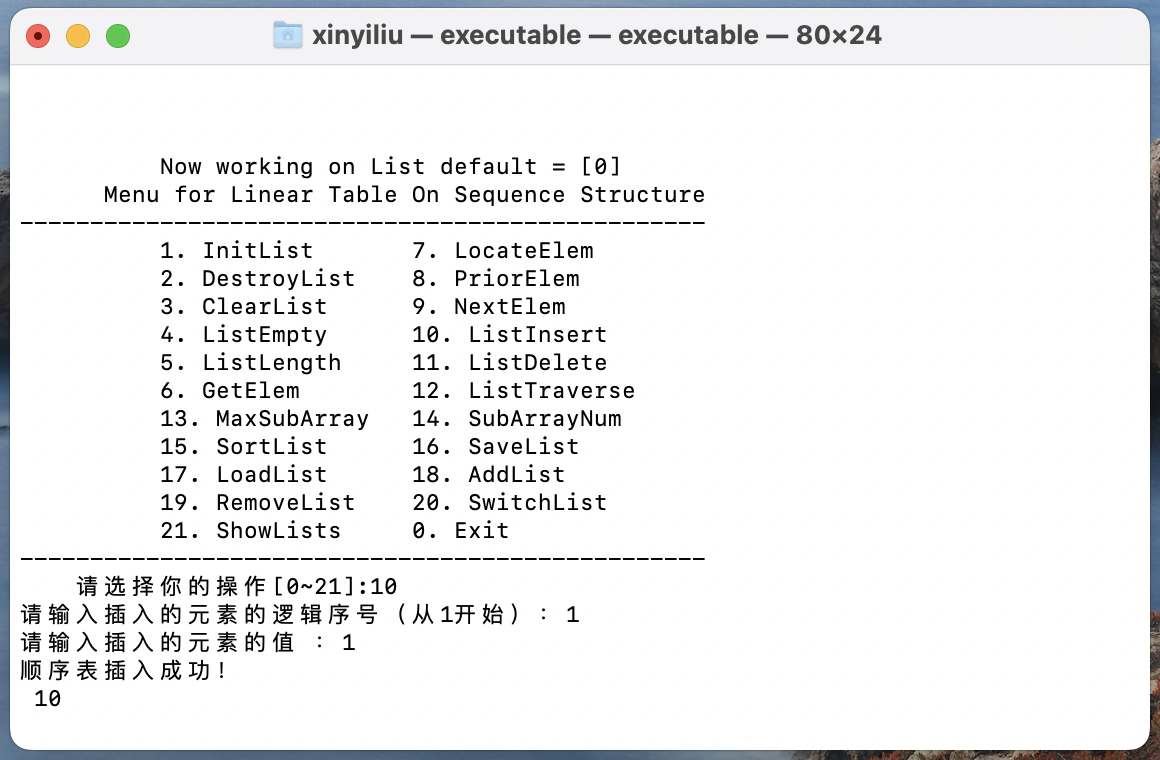
\includegraphics[width=0.8\linewidth]{images/截屏2023-06-01 18.21.51.png}
	\end{figure}
	\FloatBarrier
\newpage

\item \verb|ListEmpty()|
	\begin{figure}[!htb]
		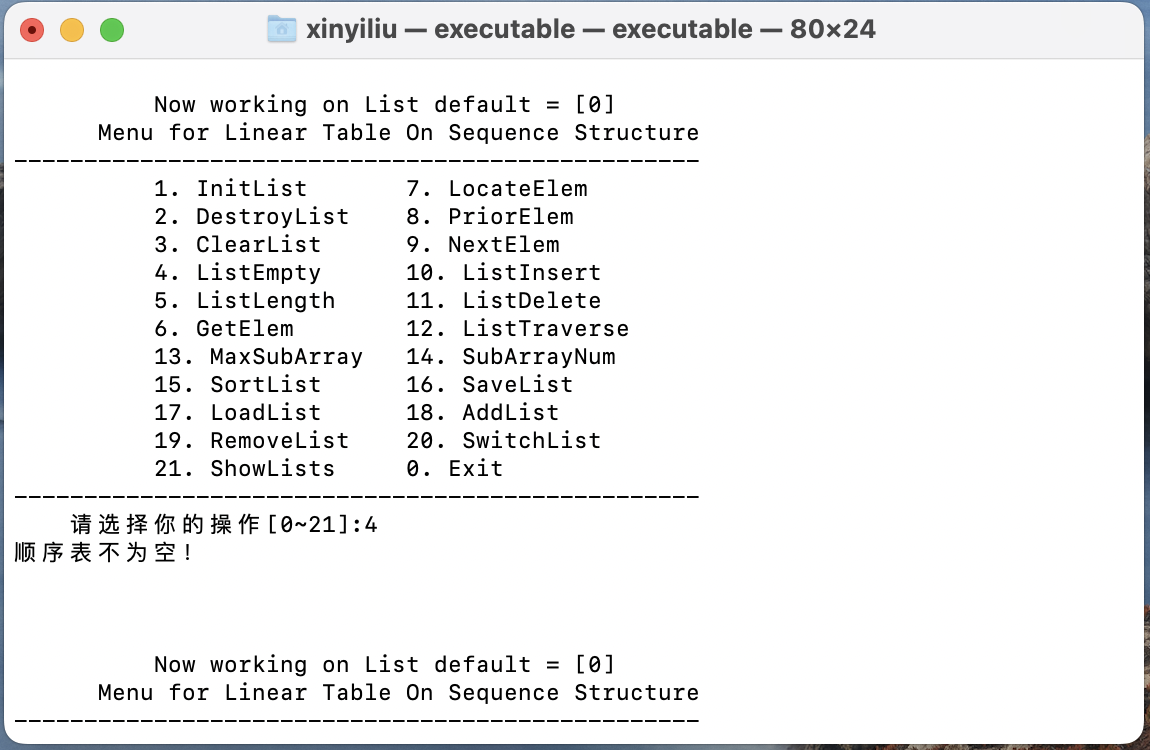
\includegraphics[width=0.8\linewidth]{images/截屏2023-06-01 18.23.33.png}
	\end{figure}
	\FloatBarrier

\item \verb|ListLength()|
	\begin{figure}[!htb]
		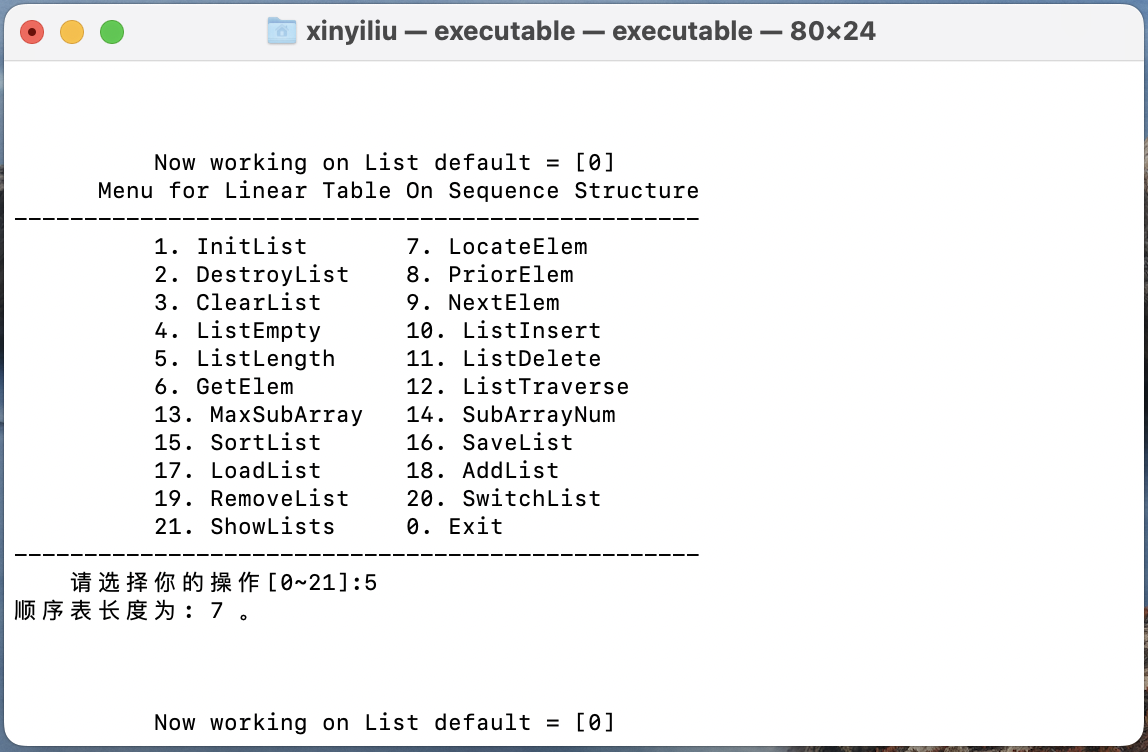
\includegraphics[width=0.8\linewidth]{images/截屏2023-06-01 18.23.42.png}
	\end{figure}
	\FloatBarrier

\newpage

\item \verb|GetElem()|
	\begin{figure}[!htb]
		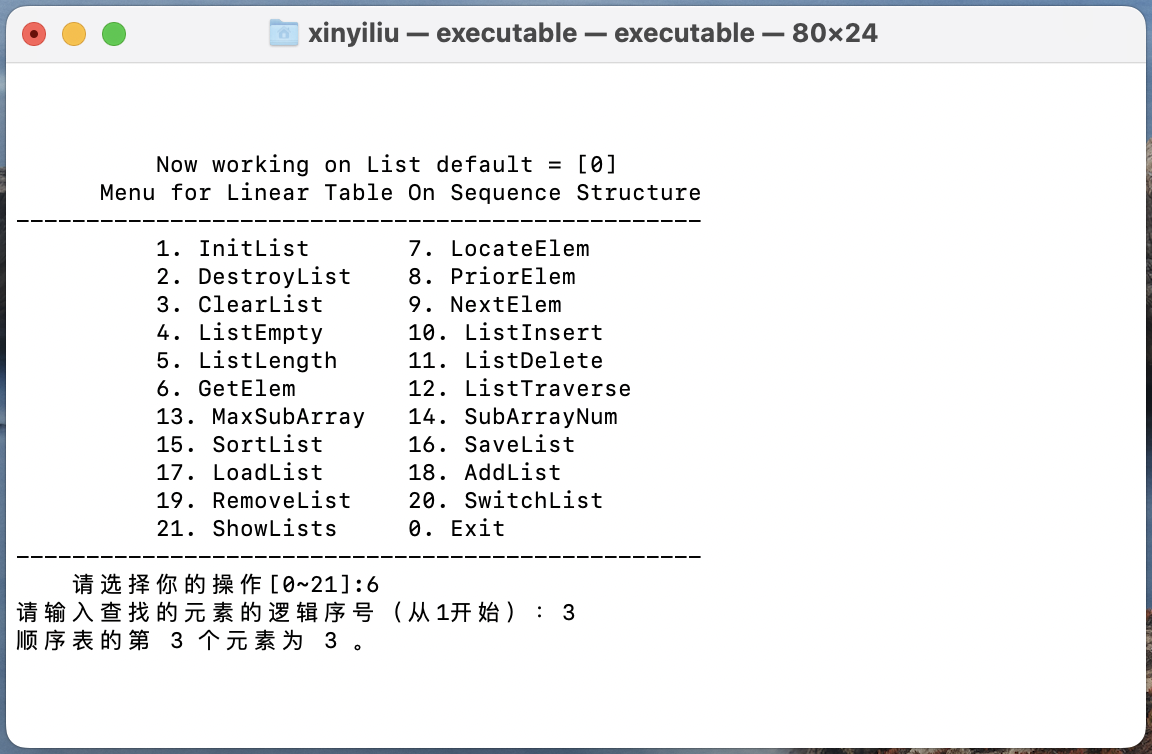
\includegraphics[width=0.8\linewidth]{images/截屏2023-06-01 18.24.07.png}
	\end{figure}
	\FloatBarrier

\item \verb|LocateElem()|
	\begin{figure}[!htb]
		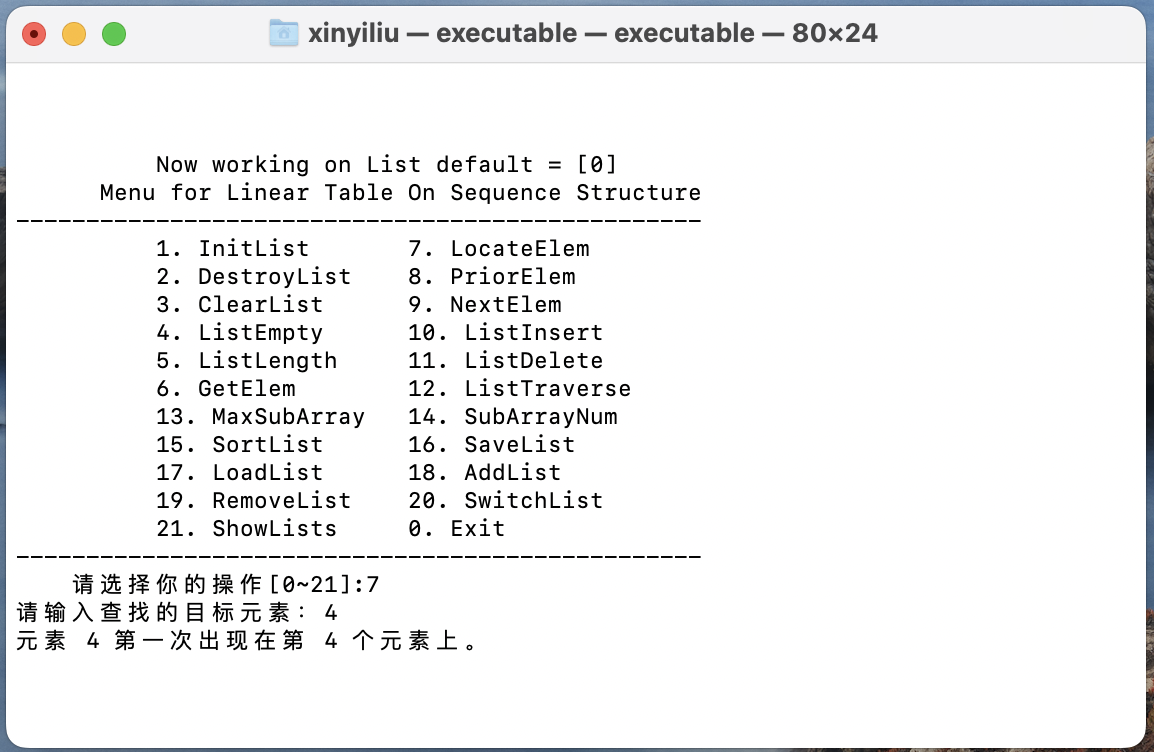
\includegraphics[width=0.8\linewidth]{images/截屏2023-06-01 18.22.44.png}
	\end{figure}
	\FloatBarrier
	
\newpage

\item \verb|PriorElem()|
	\begin{figure}[!htb]
		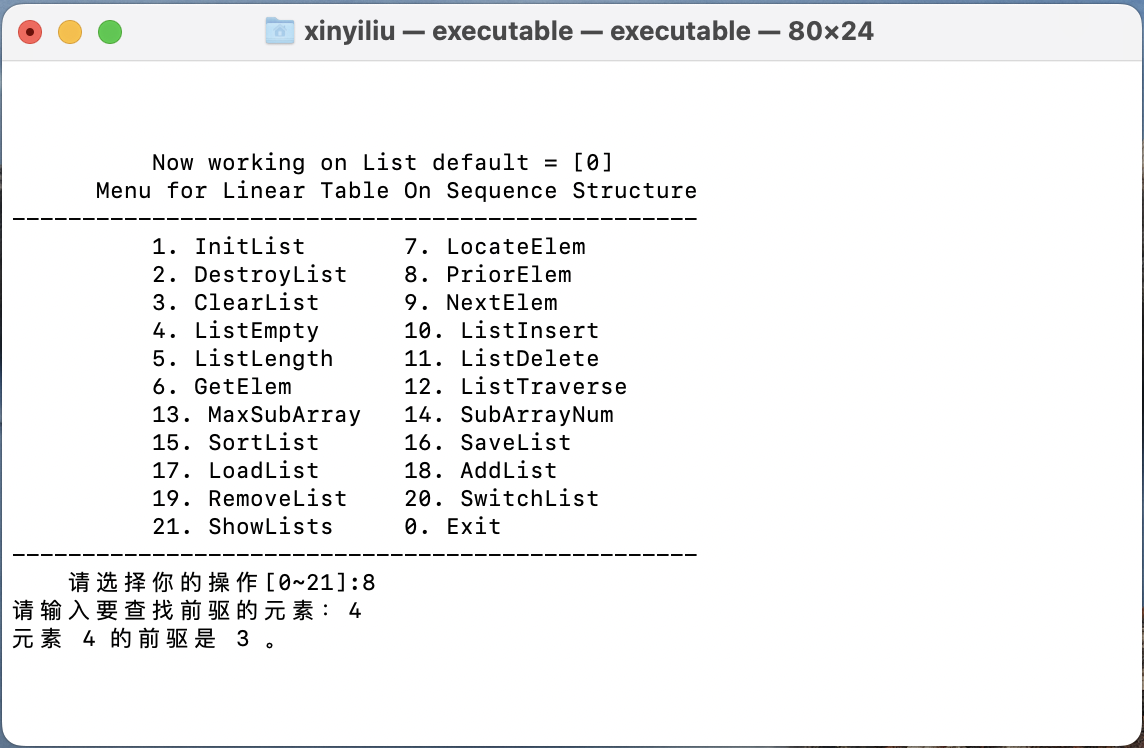
\includegraphics[width=0.8\linewidth]{images/截屏2023-06-01 18.22.56.png}
	\end{figure}
	\FloatBarrier

\item \verb|NextElem()|
	\begin{figure}[!htb]
		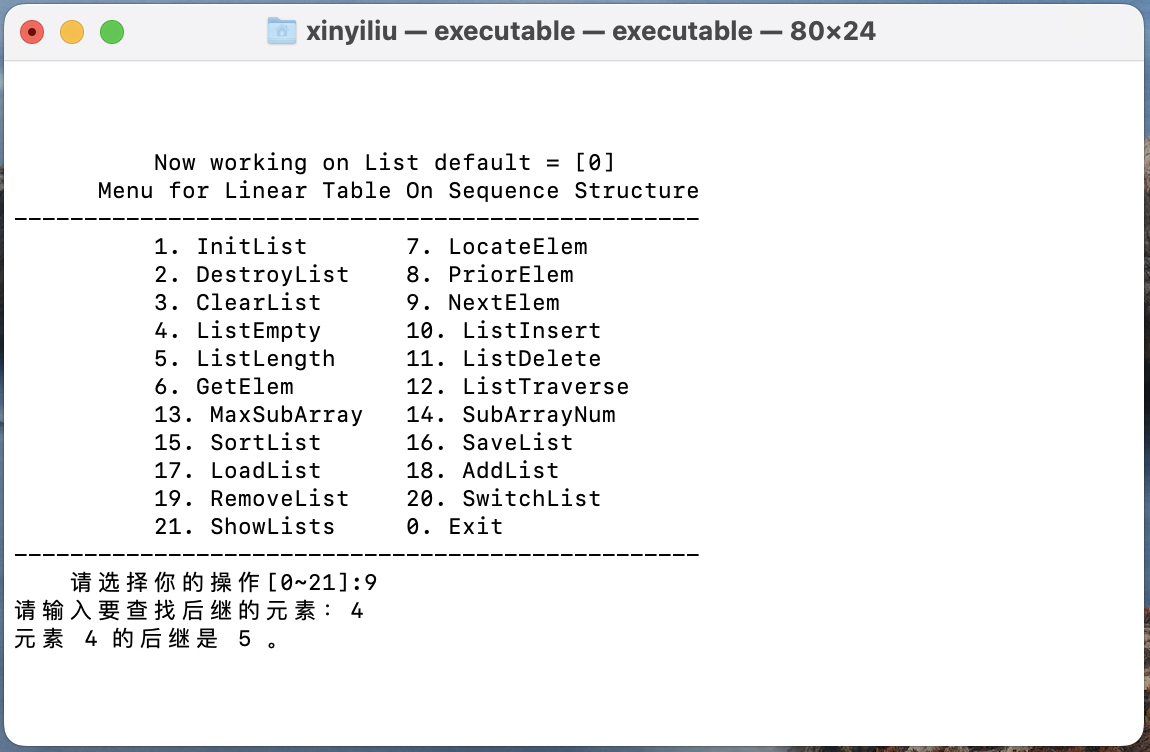
\includegraphics[width=0.8\linewidth]{images/截屏2023-06-01 18.23.17.png}
	\end{figure}
	\FloatBarrier
	
\newpage

\item \verb|ListDelete()|
	\begin{figure}[!htb]
		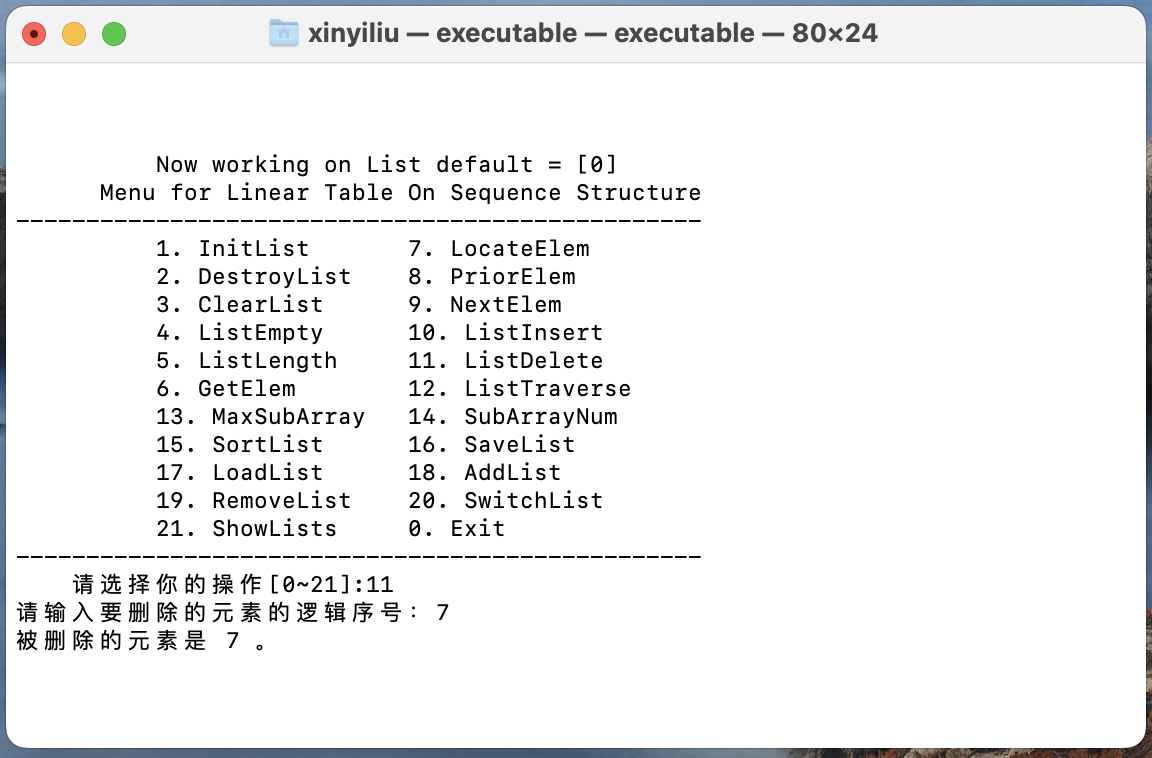
\includegraphics[width=0.8\linewidth]{images/截屏2023-06-01 18.23.53.png}
	\end{figure}
	\FloatBarrier

\item \verb|ListTraverse()|
	\begin{figure}[!htb]
		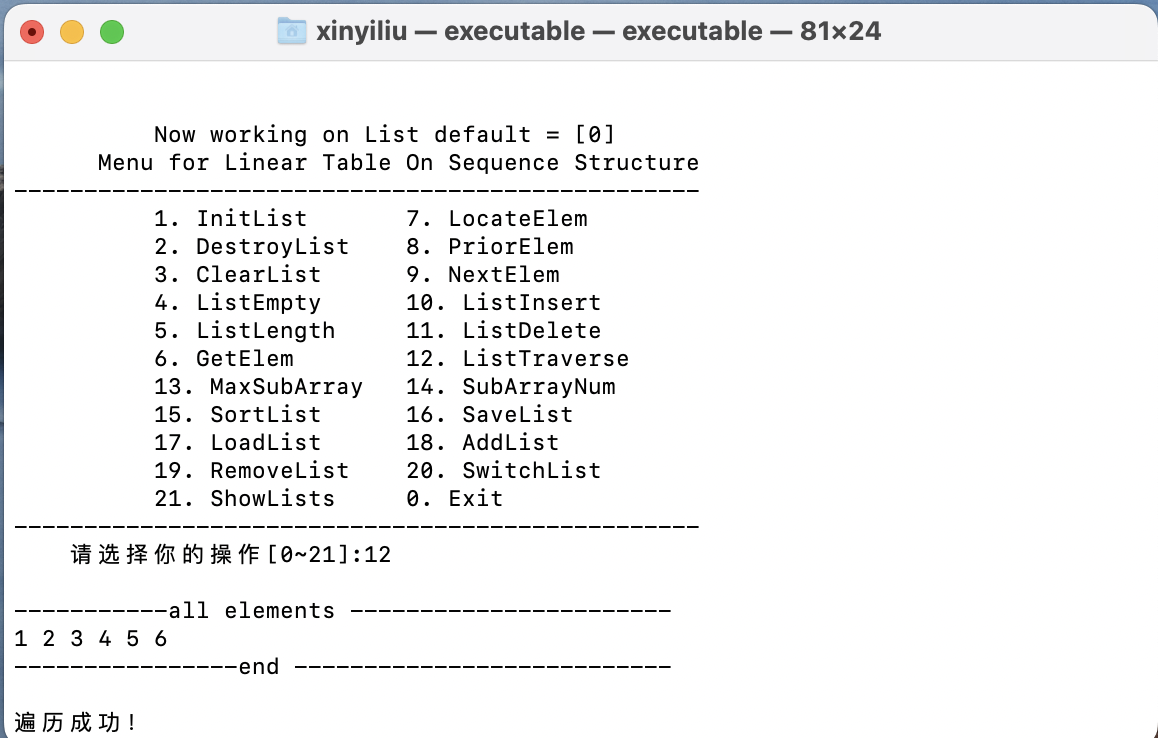
\includegraphics[width=0.8\linewidth]{images/截屏2023-06-01 21.46.52.png}
	\end{figure}
	\FloatBarrier

\newpage

\item \verb|ClearList()|
	\begin{figure}[!htb]
		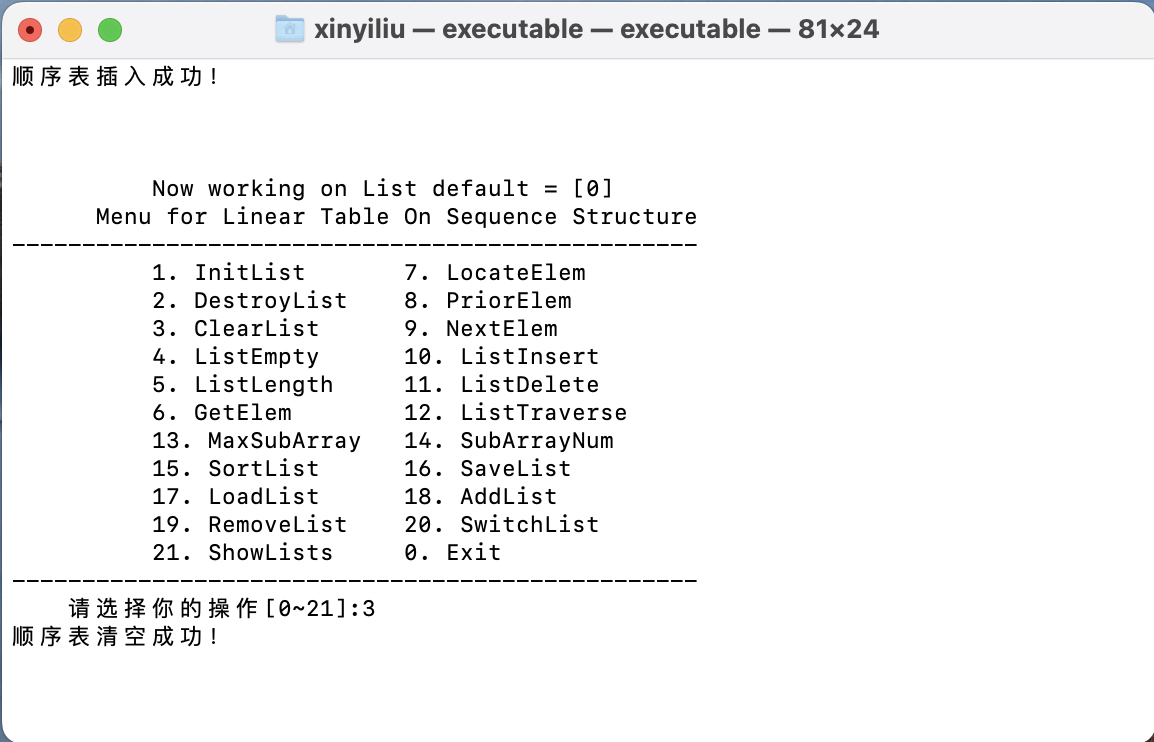
\includegraphics[width=0.8\linewidth]{images/截屏2023-06-01 21.56.17.png}
	\end{figure}
	\FloatBarrier

\item \verb|DestroyList()|
	\begin{figure}[!htb]
		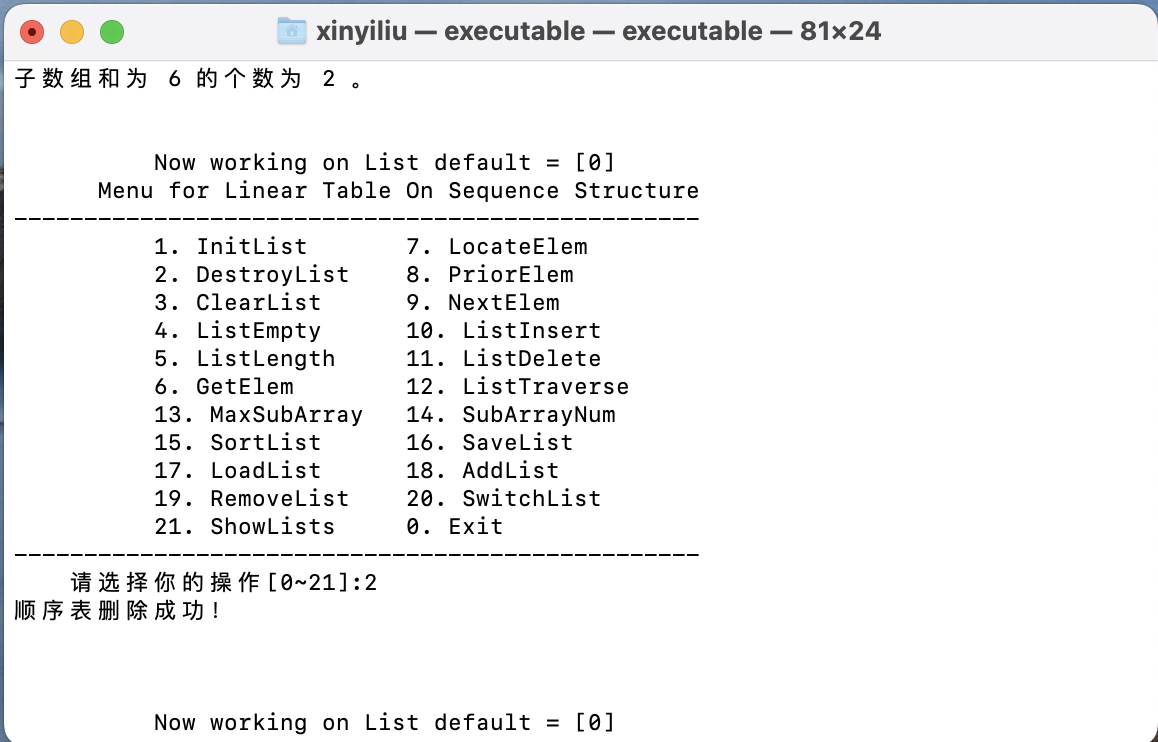
\includegraphics[width=0.8\linewidth]{images/截屏2023-06-01 18.24.43.png}
	\end{figure}
	\FloatBarrier

\end{enumerate}
\newpage

对顺序表{7,6,5,4,3,2,1}测试附加功能:
\begin{enumerate}

	\item \verb|MaxSubArray()|
	\begin{figure}[!htb]
		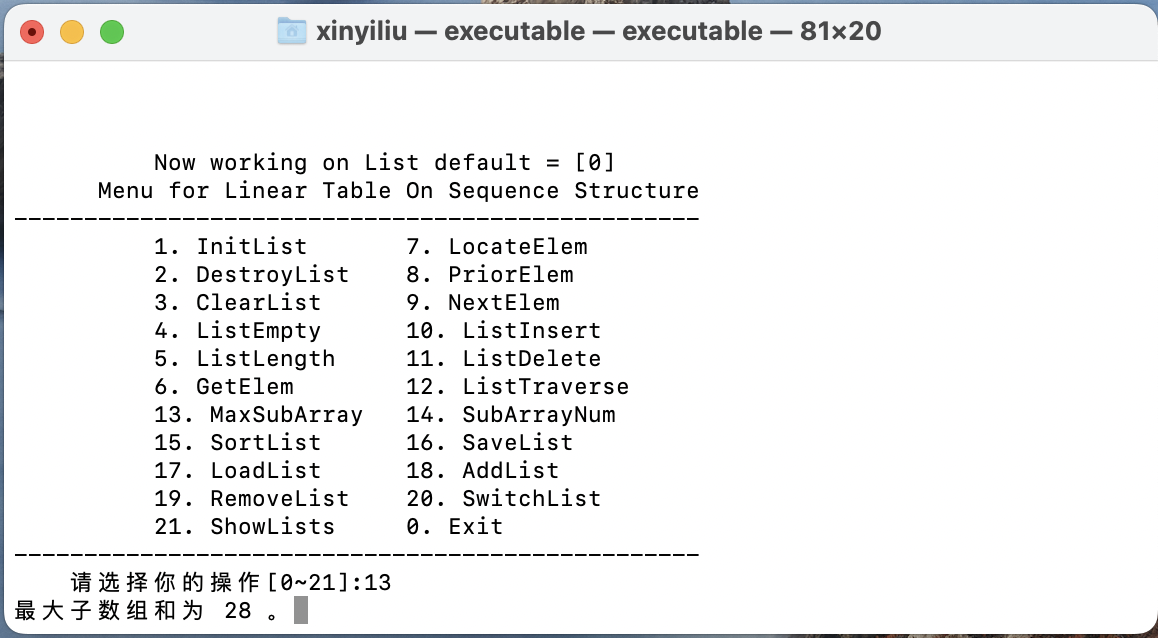
\includegraphics[width=0.8\linewidth]{images/截屏2023-06-01 22.14.26.png}
	\end{figure}
	\FloatBarrier

		
	\item \verb|SubArrayNum()|
	\begin{figure}[!htb]
		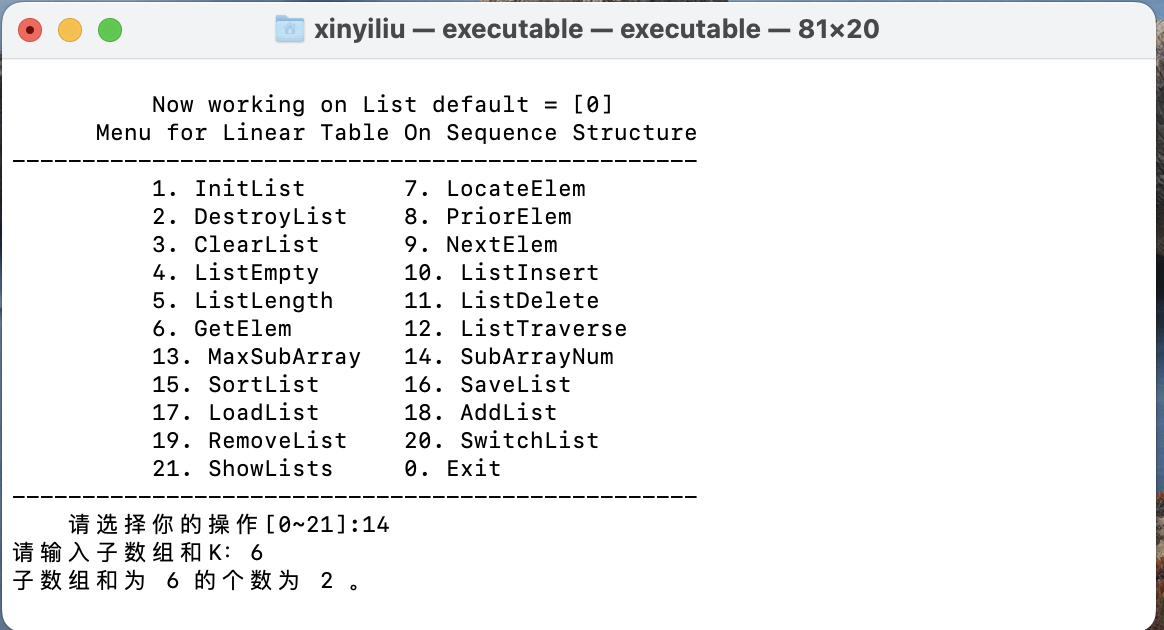
\includegraphics[width=0.8\linewidth]{images/截屏2023-06-01 22.14.44.png}
	\end{figure}
	\FloatBarrier

	\newpage

	\item \verb|SortList()|
	\begin{figure}[!htb]
		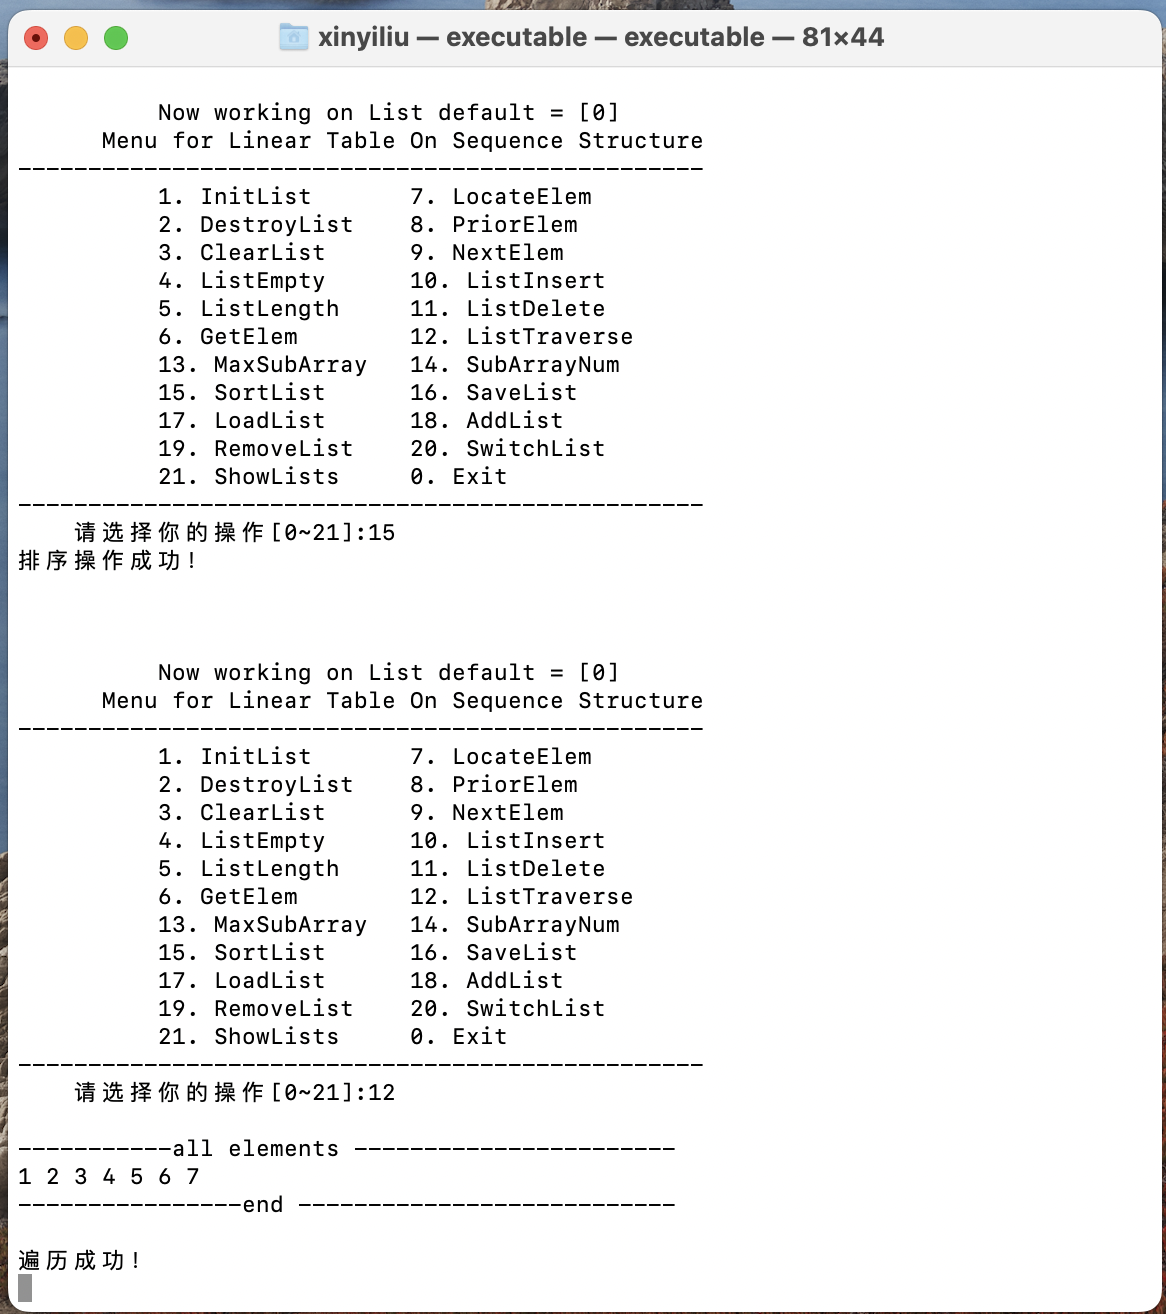
\includegraphics[width=0.8\linewidth]{images/截屏2023-06-01 22.16.47.png}
	\end{figure}
	\FloatBarrier
	
	\newpage

	\item \verb|SaveList()|、\verb|LoadList()|、\verb|List()|等多线性表管理功能。
	\begin{figure}[!htb]
		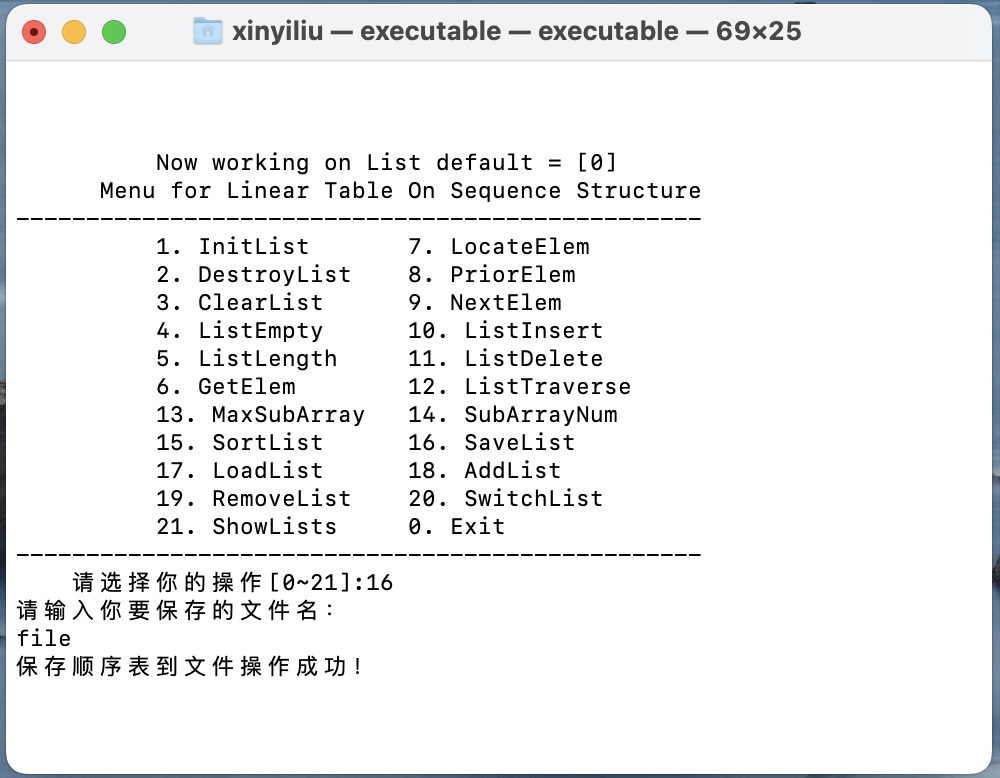
\includegraphics[width=0.8\linewidth]{images/截屏2023-06-01 22.19.25.png}
	\end{figure}
	\begin{figure}[!htb]
		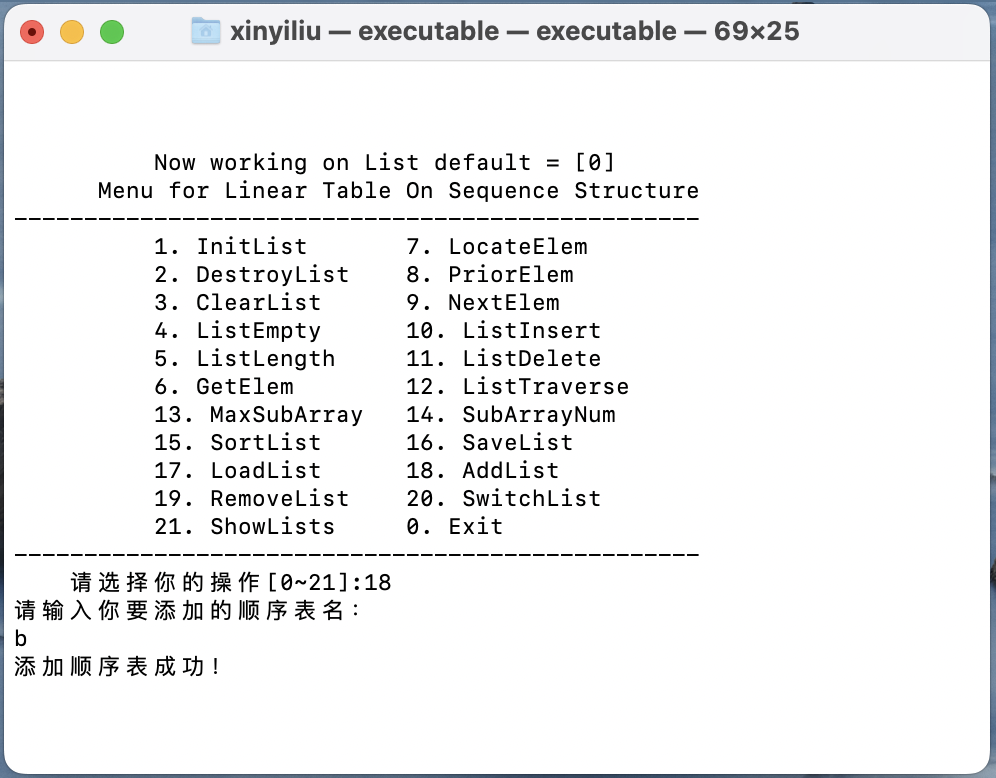
\includegraphics[width=0.8\linewidth]{images/截屏2023-06-01 22.19.36.png}
	\end{figure}
	\begin{figure}[!htb]
		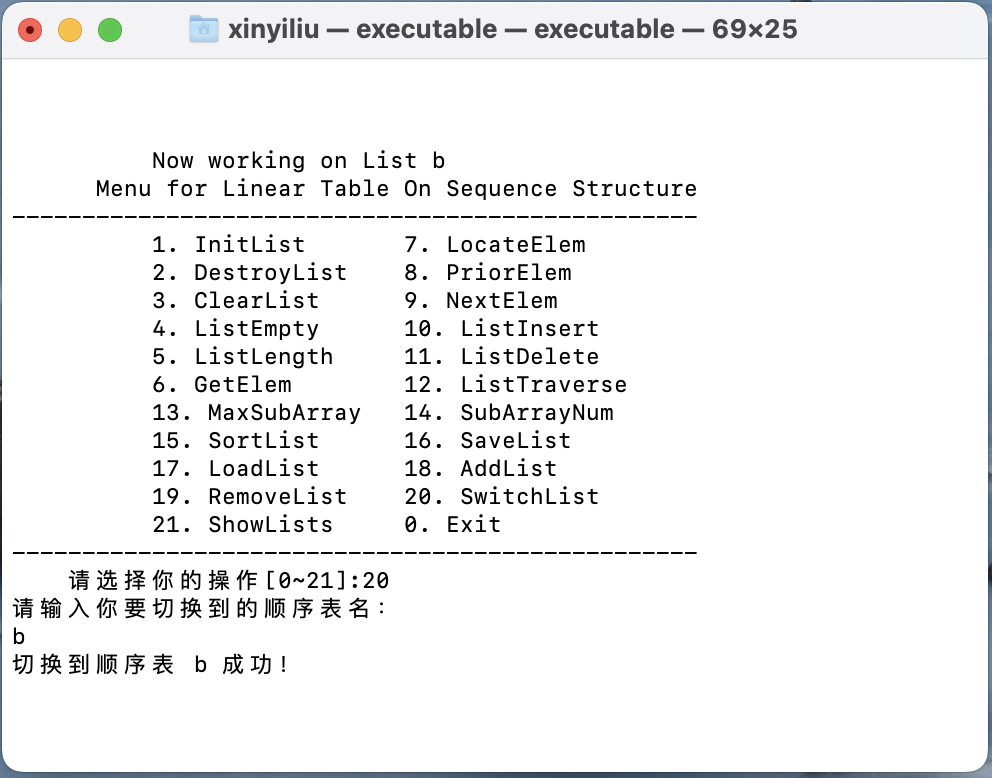
\includegraphics[width=0.8\linewidth]{images/截屏2023-06-01 22.19.46.png}
	\end{figure}
	\begin{figure}[!htb]
		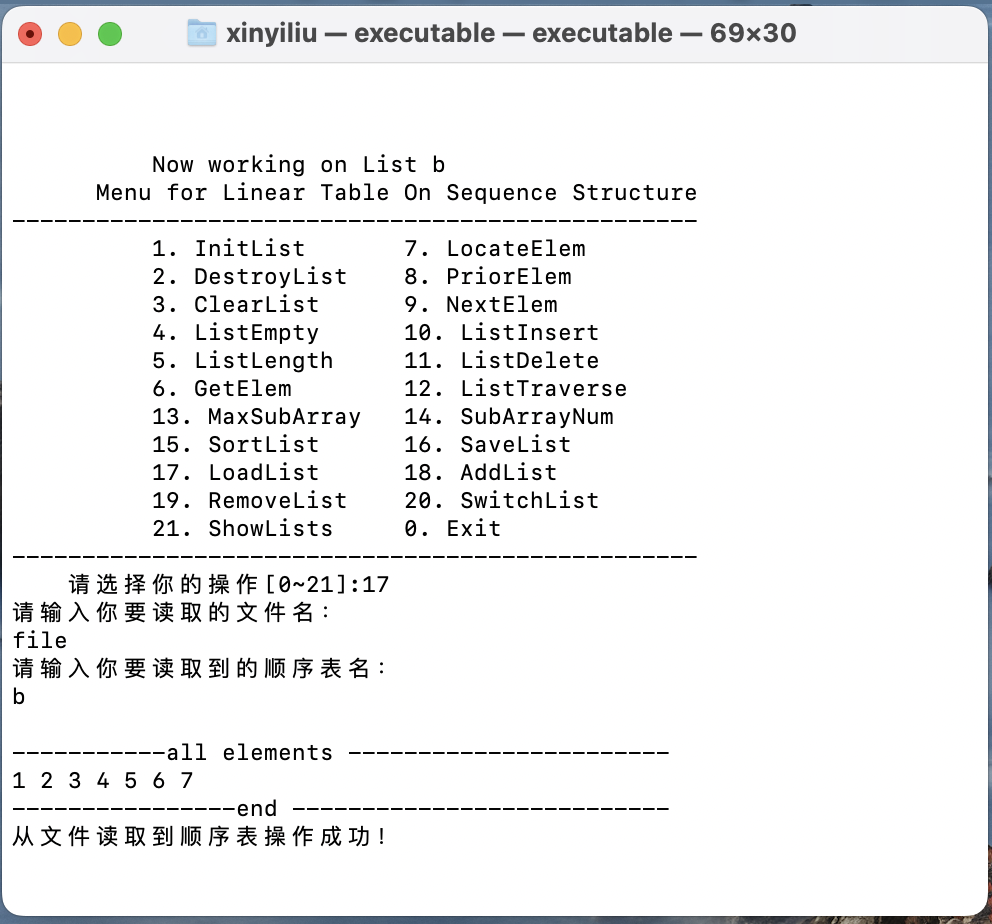
\includegraphics[width=0.8\linewidth]{images/截屏2023-06-01 22.20.01.png}
	\end{figure}
	\FloatBarrier
\end{enumerate}

\newpage
\newpage

\subsection{实验小结}
本次实验是对我C语言、数据结构知识掌握程度的一次检验。在这次实验中我发现了自己的许多不足,如对C语言文件读写的掌握不足,代码规范仍有不足。这次实验加强了我对顺序表的理解和掌握,增强的我的编写代码的能力。最后,感谢老师和助教的指导和帮助。

\newpage

\section{基于二叉链表的二叉树实现}


\subsection{问题描述}


\subsection{系统设计}


\subsection{系统实现}


\subsection{系统测试}

\subsection{实验小结}

\newpage

\section{课程的收获和建议}



\subsection{基于顺序存储结构的线性表实现}



\subsection{基于链式存储结构的线性表实现}



\subsection{基于二叉链表的二叉树实现}



\subsection{基于邻接表的图实现}


\section{附录A 基于顺序存储结构线性表实现的源程序}
\section{附录B 基于链式存储结构线性表实现的源程序}
\section{附录C 基于二叉链表二叉树实现的源程序}
\section{附录D 基于邻接表图实现的源程序}

\end{document}